\apendice{Documentación técnica de programación}

\section{Introducción}

En esta sección se describe la estructura del proyecto, el proceso de instalación y las herramientas necesarias para desarrollar el trabajo. También se explica cómo realizar la instalación de dependencias, la compilación, la ejecución del proyecto y el despliegue en Expo.

\section{Estructura de directorios}

En el primer nivel, se encuentran dos directorios, \textbf{Documentacion} y \textbf{Code}. El primero de ellos recoge los archivos de documentación sobre el proyecto, como la memoria y sus anexos, por otra parte, el segundo recoge la lógica de la aplicación.

Dentro de Code, el directorio \textbf{AppContractMe} contiene todo el código fuente necesario para la interfaz de usuario de la aplicación. Se divide en varios subdirectorios que organizan los recursos y \textit{scripts} de manera lógica, siendo \textbf{scr} el más importante, incluyendo:

\begin{itemize}

\item \textbf{AppLogin:} Contiene los componentes para la autenticación y gestión de sesiones de usuario.

\item \textbf{ContractConexion:} Incluye las funciones que facilitan la conexión y la interacción con los contratos inteligentes.

\item \textbf{Screens:} Agrupa las diferentes pantallas de la aplicación, permitiendo la navegación al usuario.

\item \textbf{components:} Reúne elementos reutilizables que se emplean en diversas partes de la aplicación, como botones y ciertas funcionalidades.

\end{itemize}

Por otro lado, también existe el directorio \textbf{SmartContract} que recoge toda la lógica del contrato inteligente e incluye:

\begin{itemize}

\item \textbf{build:} Contiene los archivos compilados de los contratos, que son necesarios para su despliegue y ejecución en la \textit{blockchain}.

\item \textbf{constracts:} Alberga los \textit{scripts} de los contratos inteligentes.

\item \textbf{migrations:} Gestiona el \textit{scripts} que ayuda en la migración y despliegue de los contratos en la \textit{blockchain}.

\item \textbf{node\_modules:} Directorio que incluye las dependencias de \texttt{Node.js} utilizadas en el proyecto.

\item \textbf{test:} Contiene los \textit{test} escritos en java para asegurar el correcto funcionamiento de los contratos inteligentes.

\end{itemize}

Finalmente hay otro directorio llamada \textbf{ganache\_db} el cual se utiliza para almacenar la configuración y los datos de la base de datos de Ganache.

Toda la jerarquía de la aplicación se puede observar en la imagen \ref{fig:FolderTree}.

\begin{figure}[h]
	\centering
	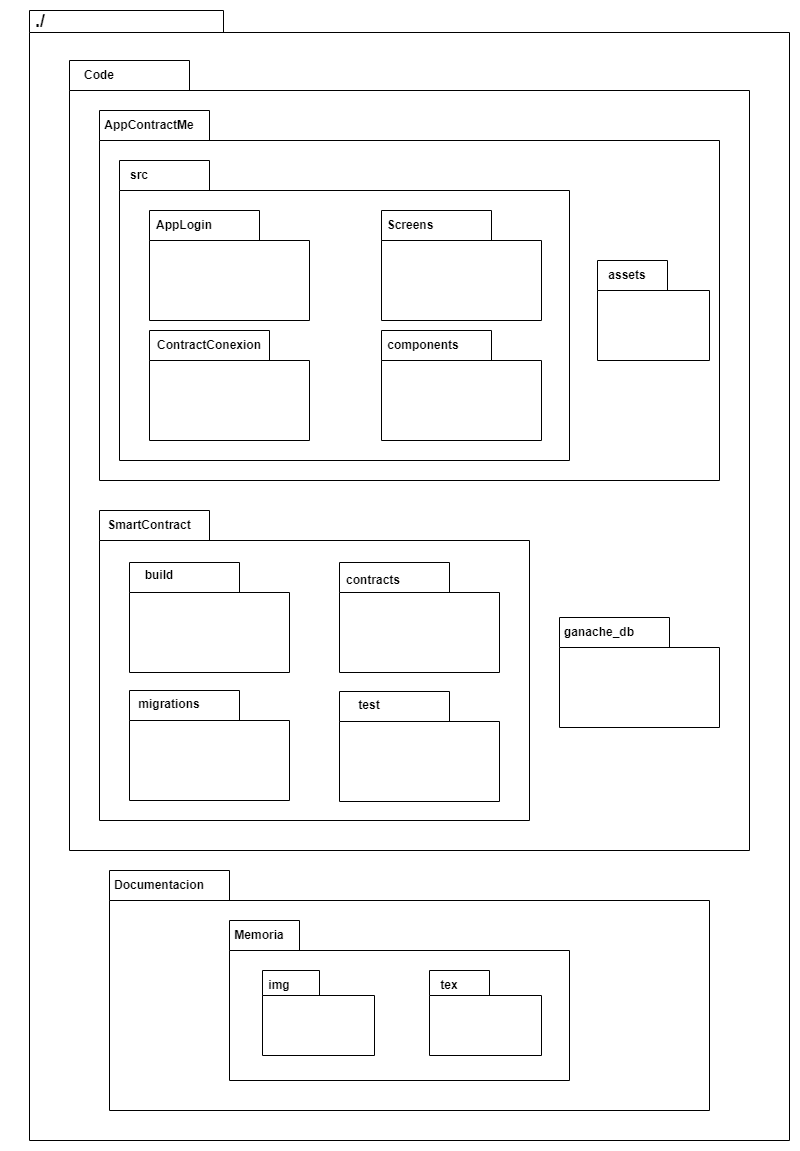
\includegraphics[width=\textwidth]{FolderTree}
	\caption[Directorios del proyecto]{Directorios del proyecto.}
	\label{fig:FolderTree}
\end{figure}


\section{Manual del programador}

Este apartado servirá de ayuda y referencia a futuros desarrolladores que quieran replicar el proyecto. 
Por ello se detallarán los requisitos necesarios y el proceso de instalación para el desarrollo de la aplicación. 

\subsection{Entorno desarrollo}

Antes de explicar la instalación de los programas y herramientas para el desarrollo de la aplicación es necesario detallar unas especificaciones mínimas en cuanto al equipo de desarrollo para poder trabajar con el proyecto.

\begin{enumerate}

\item\textbf{Procesador (CPU):}
	\begin{itemize}
	\item\textbf{Mínimo:} Procesador con arquitectura x86\_64, 2º generación de Intel o procesador AMD que
	 soporte `Hypervisor FrameWork', Permitiendo una compilación rápida de código y emular un dispositivo 	
	 móvil para pruebas.
	\item\textbf{Recomendado:} Intel Core i7 o AMD ryzen 7, con 6-8 núcleos.
	\end{itemize}
	
\item\textbf{Memoria RAM:}
	\begin{itemize}
	\item\textbf{Mínimo:} 8 GB de RAM como mínimo, para manejar diversas tareas y la ejecución de
	simuladores.
	\item\textbf{Recomendado:} 16 GB de RAM o más, pudiendo mantener múltiples dispositivos emulados
	simultáneamente.
	\end{itemize}
	
\item\textbf{Sistema operativo:}
	\begin{itemize}
	\item\textbf{Mínimo:} Windows 10 64-bit.
	\item\textbf{Recomendado:} Windows 11.
	\end{itemize}

\end{enumerate}

Por otro lado, aunque no es un requisito obligatorio, se recomienda contar con un dispositivo Android físico para ejecutar la aplicación y hacer uso de funcionalidades nativas como el reconocimiento de huella, siendo necesarias las siguientes especificaciones:

\begin{enumerate}

\item\textbf{Versión Android:}
	\begin{itemize}
	\item\textbf{Mínimo:}  Android 6.0 (Marshmallow)
	\item\textbf{Recomendado:} Android 9.0 (Pie) o superior.
	\end{itemize}
	
\item\textbf{Procesador (CPU):}
	\begin{itemize}
	\item\textbf{Mínimo:} Quad-core 1.2 GHz.
	\item\textbf{Recomendado:} Octa-core 2.0 GHz o superior.
	\end{itemize}
	
\item\textbf{RAM:}
	\begin{itemize}
	\item\textbf{Mínimo:} 2 GB de RAM.
	\item\textbf{Recomendado:} 4-8 GB de RAM.
	\end{itemize}
	
\item\textbf{Compatibilidad con características nativas:}
	\begin{itemize}
	\item\textbf{Huella digital:} El dispositivo debe contar con un sensor de huellas dactilares compatible con
	las API de Android para autenticación biométrica.
	\item\textbf{Reconocimiento facial:} cámara interior con capacidad de reconocimiento facial.
	\item\textbf{Cámara trasera:} Cámara de al menos 8 MP para la lectura de códigos QR.
	\end{itemize}

\end{enumerate}


\section{Compilación, instalación y ejecución del proyecto}

\subsection{Instalación}

Seguidamente se detallará como configurar un entorno de desarrollo para poder trabajar en la aplicación ContractMe.

\begin{enumerate}

\item \textbf{Node.js:} Node.js es una plataforma de ejecución para JavaScript del lado del servidor y es esencial para la gestión de paquetes y la ejecución de varias herramientas de desarrollo. 
Para instalar Node.js es necesario dirigirse a la \href{https://nodejs.org/en}{pagina oficial de Node.js} y seleccionar el instalador para Windows. Ver imagen \ref{fig:InstalarNodejs}.

Al ejecutar el instalador que se ha descargado, es necesario seleccionar la opción que permite instalar npm y añadir Node.js a tu \textit{path}. Ver imagen \ref{fig:NodejsSetUp}.  
En concreto la versión utilizada de Node.js para el desarrollo del proyecto ha sido la v18.18.2 y la versión utilizada de npm ha sido la 10.2.2.

\begin{figure}[h]
	\centering
	\includegraphics[width=\textwidth]{InstalarNodejs}
	\caption[Descarga de Node.js]{Descarga de Node.js.}
	\label{fig:InstalarNodejs}
\end{figure}

\begin{figure}[h]
	\centering
	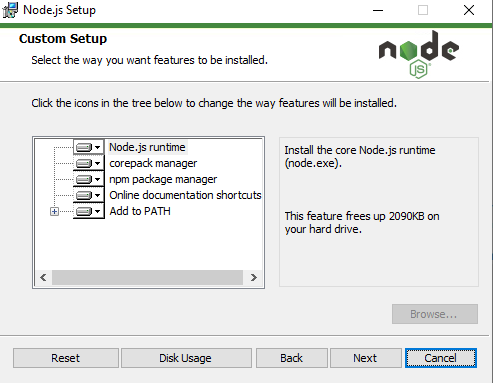
\includegraphics[width=\textwidth]{NodejsSetUp}
	\caption[Instalar Node.js y npm]{Instalar Node.js y npm.}
	\label{fig:NodejsSetUp}
\end{figure}

\item \textbf{Truffle Suite}: Teniendo Node.js y npm instalados, procederemos a instalar Truffle globalmente, para ello desde la terminal ejecutaremos el siguiente comando: \texttt{npm install -g truffle} lo cual nos permitirá usar el comando \texttt{truffle} desde cualquier lugar en la terminal.

Una vez instalado Truffle, el siguiente paso es configurar el proyecto, para ello dentro del directorio \textit{Smart Contract}, se encuentra la estructura de carpetas generadas por Truffle, incluyendo \textit{contracts} para almacenar la lógica de los contratos, \textit{migrations} para almacenar el \textit{migrations} de migración y \textit{test} para las pruebas.

Truffle también crea un archivo llamado \texttt{truffle-config.js}, el cual se usa para configurar las redes sobre las cuales se desplegarán los contratos inteligentes.
En este caso se usa la red de Ganache, que normalmente se ejecuta en \texttt{localhost} en el ordenador. Debido a que la aplicación se ejecutará en un dispositivo móvil independiente del ordenador, la configuración \textit{localhost} no será suficiente. 
En su lugar, se usará la dirección IP del ordenador la cual actuará como servidor para Ganache. Esto permitirá que otros dispositivos de nuestra misma red local se conecten a la \textit{blockchain} simulada por Ganache.
Ganache por defecto usa el puerto 8545, aunque este podría ser reemplazado por cualquier puerto que se encontrase vacío.
Siguiendo los pasos previamente mencionados, el archivo \texttt{truffle-config.js} debería verse como en la imagen \ref{fig:TruffleGanache}.

\begin{figure}[h]
	\centering
	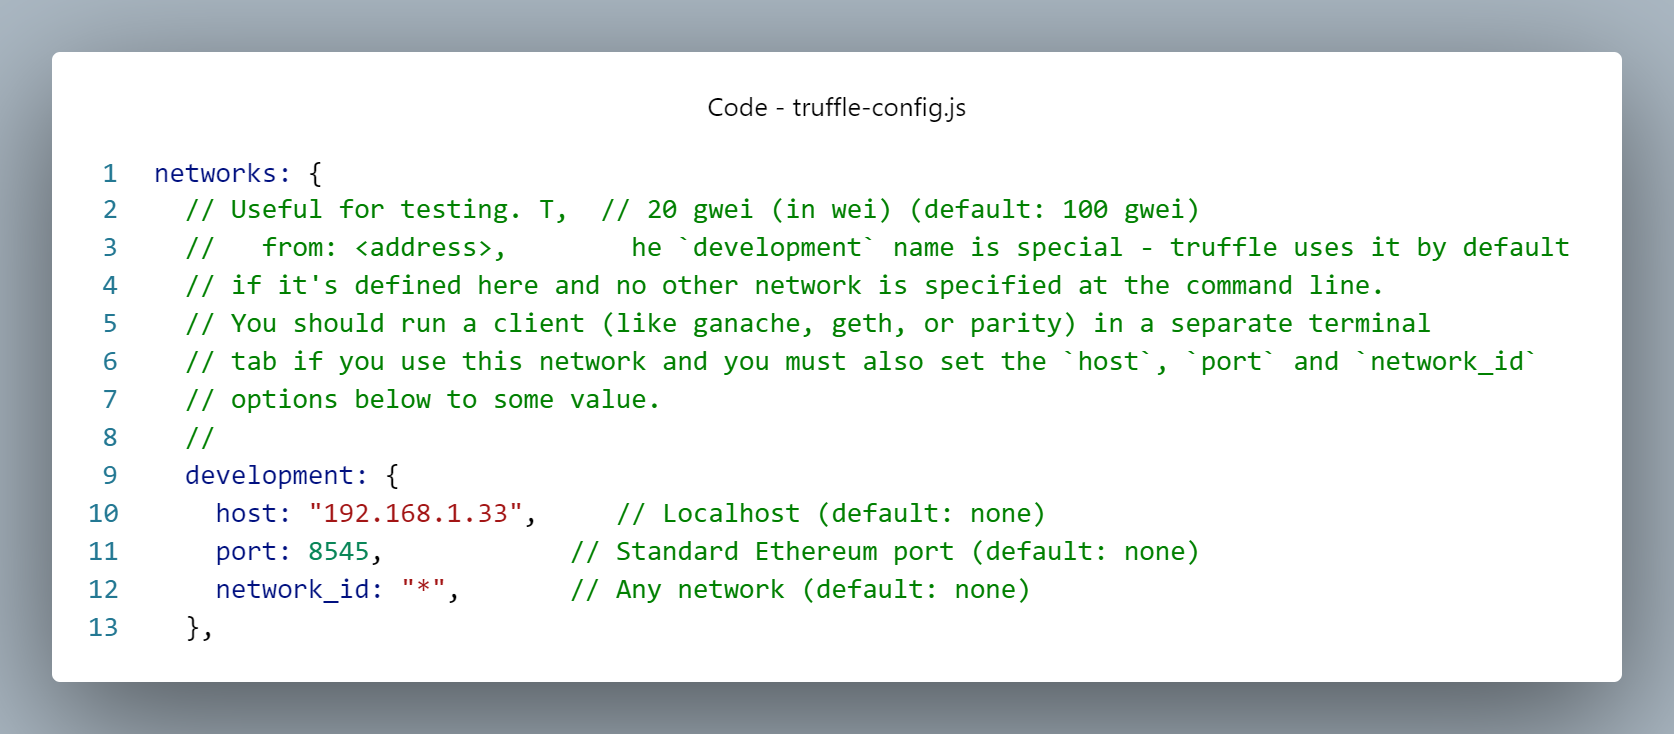
\includegraphics[width=\textwidth]{TruffleGanache}
	\caption[Configuración Ganache Truffle]{Configuración red Ganache en truffle-config.js.}
	\label{fig:TruffleGanache}
\end{figure}

Dentro del archivo \texttt{truffle-config.js} también será necesario realizar la configuración de compiladores para especificar como los contratos inteligentes deben de ser compilados, optimizados y ejecutados en la máquina virtual de Ethereum.
Se deberá especificar la versión \textbf{0.8.20}, la cual usará Truffle para compilar los contratos, esta versión coincide con la versión que se ha usado de Solidity para desarrollar los contratos inteligentes.
Dentro de \textit{Settings} se ha de especificar algunas opciones que afectan a la compilación de los contratos. La opción \textit{optimizer} debe marcarse como \textit{true}, ayudándonos a reducir el código \textit{byte} de los contratos y hacerlos más eficientes en términos de gas.
Por otro lado, las \textit{runs} se deben de establecer en 200, un número más alto puede resultar en un código más optimizado en términos de gas, pero con un proceso de compilación más lento. ver imagen \ref{fig:TruffleCompiler}.

\begin{figure}[h]
	\centering
	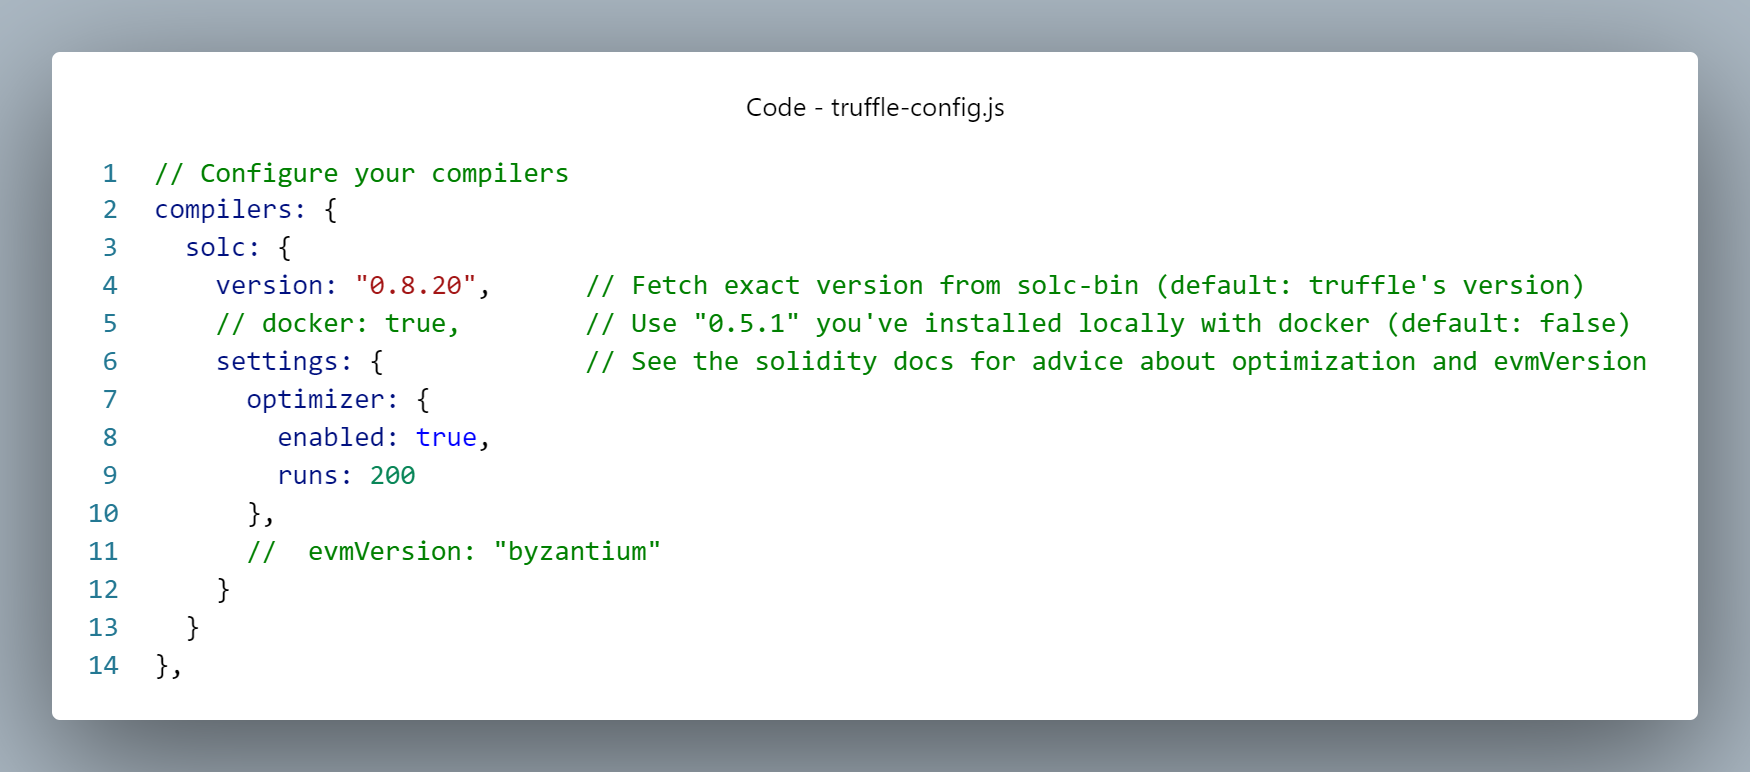
\includegraphics[width=\textwidth]{TruffleCompiler}
	\caption[Configuración compilador Truffle]{Configuración del compilador en truffle-config.js.}
	\label{fig:TruffleCompiler}
\end{figure}

\item \textbf{Ganache}: Como hemos comentado, en el proyecto se usa la red de Ganache. Por simplicidad hemos usado la versión de consola, por tanto para instalarla de forma global en nuestro ordenador será necesario ejecutar el siguiente comando: \texttt{npm install -g ganache-cli}.

\item \textbf{Expo CLI}: Del mismo modo que hemos realizado con Ganache, previamente es necesario descargar Expo CLI, el cual es necesario para iniciar, desarrollar y probar el proyecto.
Utilizando el comando \texttt{npm install -g expo-cli} lo descargamos globalmente.

\item \textbf{Expo Go}: Para visualizar la aplicación se usará Expo Go permitiéndonos ejecutar la aplicación directamente en nuestra dispositivo móvil.
Para ello, desde el un dispositivo móvil Android utilizando Google Play Store, se buscará en la barra de búsqueda `Expo Go'.  Seguidamente se procederá a descargar dicha aplicación.

\item \textbf{Descarga del repositorio}: Para adquirir el código fuente del proyecto \href{https://gitlab.com/HP-SCDS/Observatorio/2023-2024/contractme/ubu-contractme.git}{`ContracMe'}, se puede descargar de utilizando la interfaz gráfica de GitLab descargando el fichero ZIP o usando \texttt{git clone} desde la terminal.

\end{enumerate}


\subsection{Ejecución del proyecto}

En este apartado se detallará cómo ejecutar el proyecto. Es muy importante que durante la ejecución tanto el ordenador como el dispositivo móvil se encuentren en la misma red.

\begin{enumerate}

\item \textbf{Levantar Ganache}: Antes de proceder a ejecutar la aplicación es necesario que la red Ganache se encuentre previamente en funcionamiento.
Como hemos comentado anteriormente, la red debe de ser levantada sobre la dirección IP local de nuestro ordenador. Por ejemplo, suponiendo que la IP local de mi ordenador es 192.168.1.33, deberemos de ejecutar desde cualquier parte de la terminal, el siguiente comando: 
\begin{verbatim}
ganache-cli --host 192.168.1.33 -d --db ganache_db
\end{verbatim}

\texttt{-d} es una abreviatura de deterministic, lo que hace que Ganache genere las mismas cuentas y claves privadas cada vez que se ejecuta.
\texttt{--db ganache\_db} es una opción que permite que Ganache guarde el estado de la red en un directorio específico, en este caso el directorio será llamado `ganache\_db' y se creará en la rama actual donde se encuentre el usuario en la terminal.
Esto permite que la \textit{blockchain} simulada mantenga su estado entre reinicios de Ganache.

En la imagen \ref{fig:ganache-cli} se muestra el resultado de levantar exitosamente una red Ganache desde la terminal.

\begin{figure}[h]
	\centering
	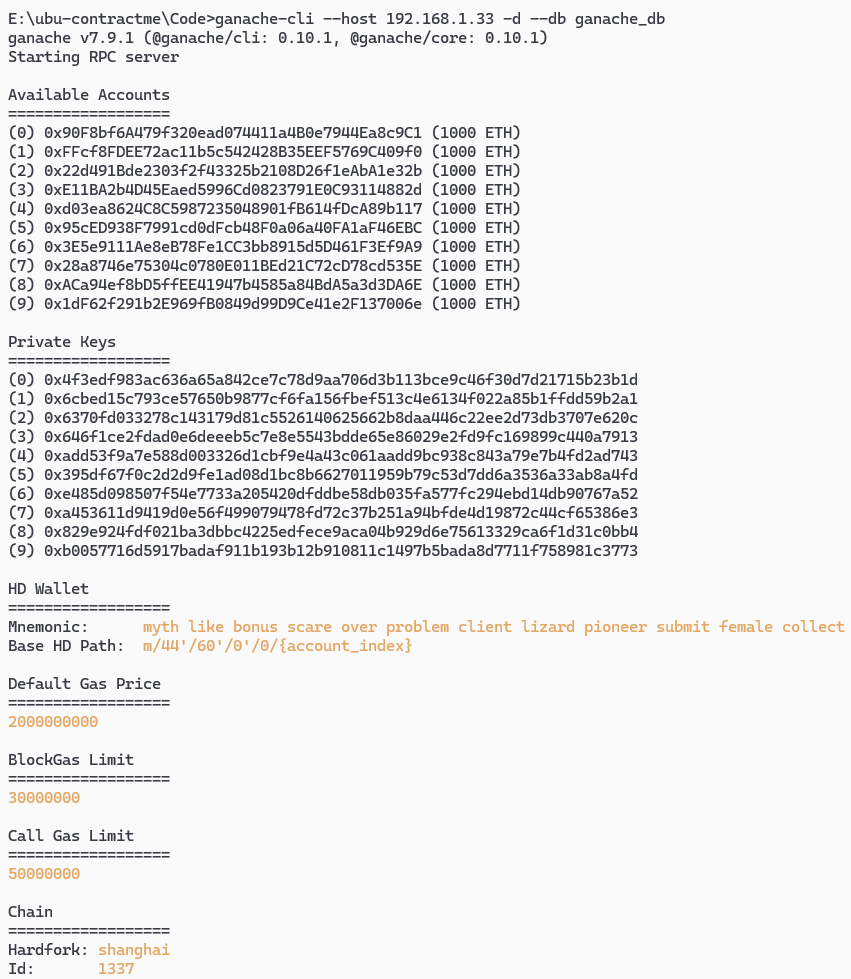
\includegraphics[width=\textwidth]{ganache-cli}
	\caption[Levantar red Ganache]{Levantar red local usando Ganache.}
	\label{fig:ganache-cli}
\end{figure}

\item \textbf{Compilar y migrar contrato}: el contrato debe de ser compilado, probado y migrado antes de poder utilizarlo, para ello se utiliza Truffle.

	\begin{itemize}
	\item \textbf{Compilar}: Es necesario convertir el código
	Solidity de los contratos en \textit{bytecode} que pueda
	ser ejecutado por la Máquina Virtual de Ethereum (EVM).
	Para ello desde el directorio \textit{SmartContract} donde se
	almacena toda la lógica de los contratos
	inteligentes, se debe ejecutar el comando \texttt{truffle
	compile}.
	Ver imagen \ref{fig:TruffleCompile}.
	\end{itemize}
	
\begin{figure}[h]
	\centering
	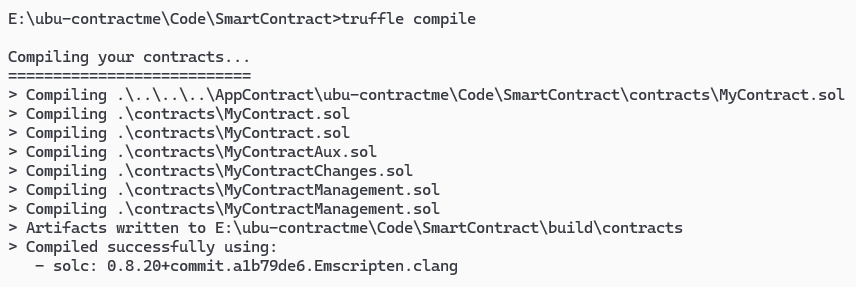
\includegraphics[width=\textwidth]{TruffleCompile}
	\caption[Compilar smart contract]{Compilar \textit{smart contract} usando Truffle.}
	\label{fig:TruffleCompile}
\end{figure}	
	
	\begin{itemize}
	\item \textbf{Migrar}: Finalmente, el último paso es desplegar el contrato en la \textit{blockchain}.
	Esto se realiza desde el directorio \texttt{SmartContract} usando el comando \texttt{truffle migrate}.
	Este comando desplegará los contratos inteligentes en la red configurada, en este caso Ganache y generará
	los archivos necesarios en el directorio \texttt{build/contracts}.
	Tras una correcta migración, se mostrará la dirección del contrato, la cuenta del creador, el costo total
	del despliegue, etcétera. 	
Ver imagen \ref{fig:TruffleMigrate}.
	\end{itemize}
	
\begin{figure}[h]
	\centering
	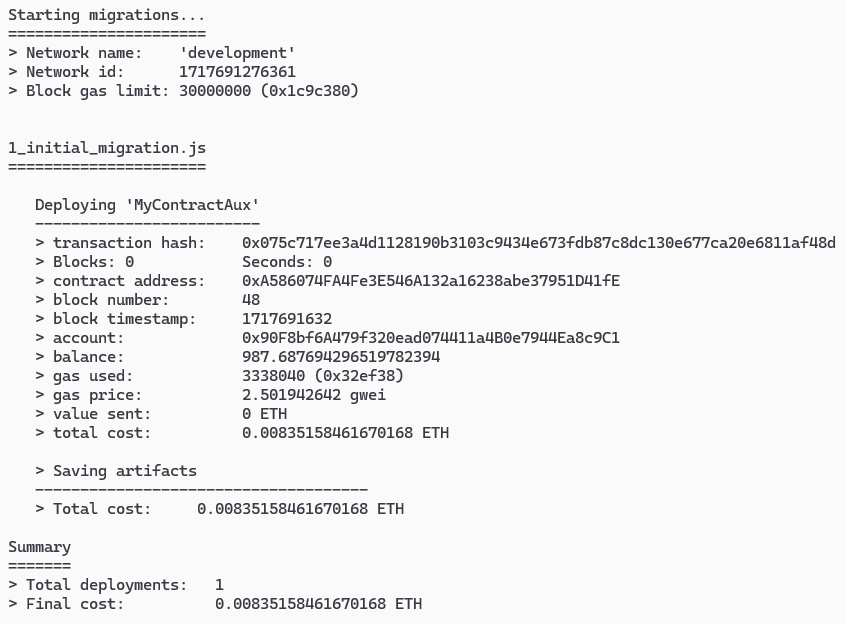
\includegraphics[width=\textwidth]{TruffleMigrate}
	\caption[Despliegue smart contract]{Despliegue del contrato en la red de Ganache usando Truffle.}
	\label{fig:TruffleMigrate}
\end{figure}	
	
	
\item \textbf{Configuración conexión contrato}: Una vez hayamos desplegado un nuevo contrato en la \textit{blockchain}, debemos actualizar la información de la aplicación para que esta pueda interactuar con él.
Para ello, necesitamos dos cosas: la dirección del contrato, que se nos ha proporcionado en la terminal al migrarlo, y el archivo JSON del contrato que se encuentra en \texttt{SmartContract/build}.
	
Con el archivo JSON del contrato, es necesario copiarlo y pegarlo en la carpeta \texttt{AppContract/src/ContractConexion}. 
Por otro lado, con la dirección del contrato, también es necesario copiarla, y actualizar la referencia \texttt{contractAddress} que se encuentra en el archivo \texttt{EtherProvider.js}.
Ver imagen \ref{fig:ContractConexion}.

\begin{figure}[h]
	\centering
	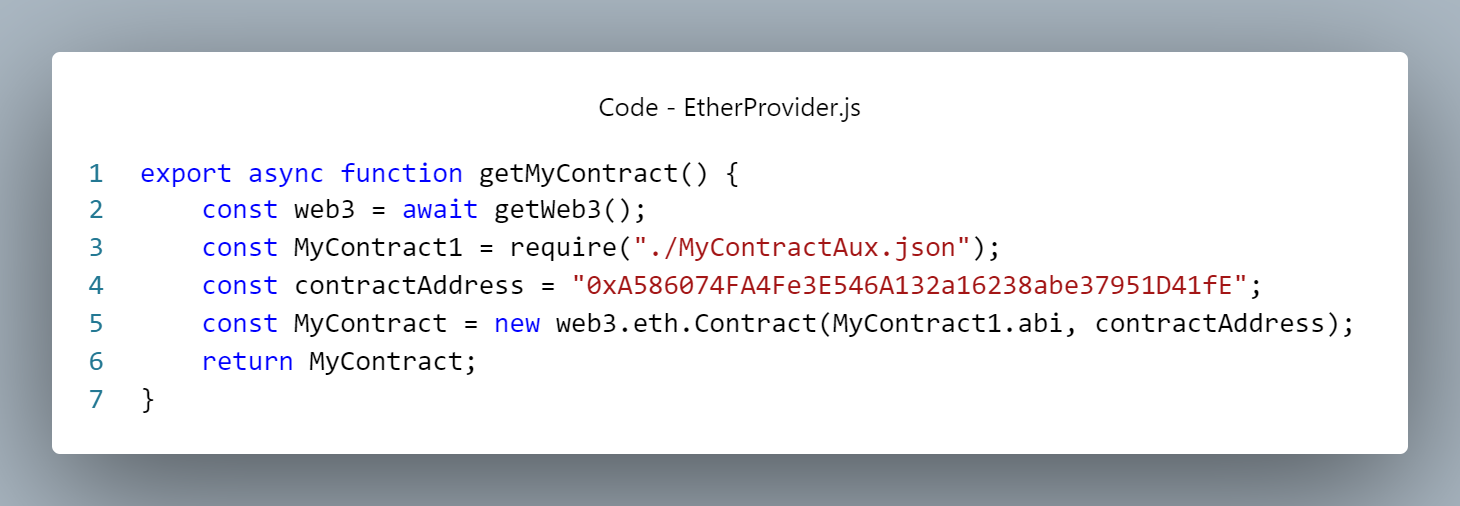
\includegraphics[width=\textwidth]{ContractConexion}
	\caption[Conexión con el contrato]{Configuración de conexión con el contrato.}
	\label{fig:ContractConexion}
\end{figure}	

\item \textbf{Iniciar aplicación}: Desde el directorio raíz, \texttt{/Code/AppContract}, en la terminal ejecutamos el comando \texttt{npx expo start} para iniciar el servidor. Esto mostrará un código QR en la terminal. Será necesario comprobar que la opción Expo Go se encuentre activa.
Seguidamente desde la aplicación Expo Go en el dispositivo móvil, se procederá a escanear el código QR que aparece en la terminal.
La aplicación Expo Go cargará y mostrará la aplicación en el dispositivo móvil.

\end{enumerate}

\section{Pruebas del sistema}

\begin{itemize}

\item \textbf{Probar}: Como paso opcional, pero altamente recomendado, para comprobar el correcto funcionamiento del contrato, se puede ejecutar una batería de \textit{test}. Estos \textit{tests} están diseñados para asegurar que todas las funciones del contrato inteligente operen conforme a las especificaciones establecidas y para identificar cualquier posible falla antes de la implementación en un entorno de producción.
	
\item \textbf{Proceso de ejecución de pruebas}: Para llevar a cabo estas pruebas unitarias, es necesario utilizar el comando \texttt{truffle test} en la terminal. Este comando debe ejecutarse desde el directorio \textit{Smart Contract}, donde se encuentran almacenados todos los \textit{scripts} de prueba necesarios para la evaluación del contrato.

\item \textbf{Descripción de los \textit{tests}}: 
Los \textit{tests} verifican cada función y transacción que el
contrato inteligente puede realizar, incluyendo la creación,
transferencia y administración de los contratos.
Cada \textit{test} está diseñado para garantizar que el contrato responda adecuadamente en cualquier situación.

\item \textbf{Interpretación de resultados}: Al finalizar la ejecución de los \textit{test}, \texttt{truffle} proporcionará un reporte detallado que incluirá el resultado de cada prueba individual.
Un \textit{test} exitoso indica que la función correspondiente del contrato cumple con los requisitos y funciona como se espera. 
Para ver un ejemplo de cómo se presentan estos resultados, ver la imagen \ref{fig:TruffleTest}.

\end{itemize}

\begin{figure}[h]
	\centering
	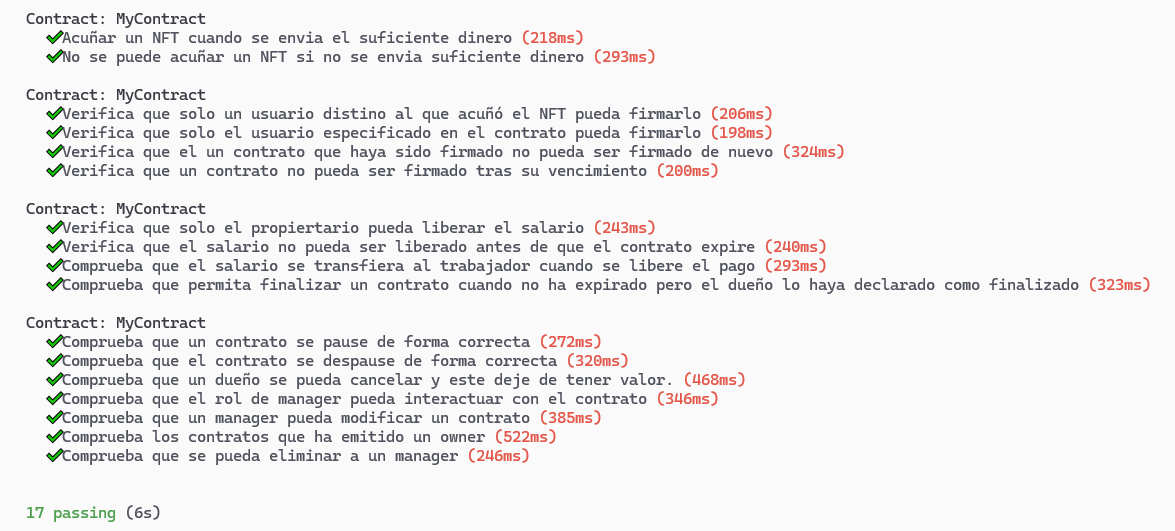
\includegraphics[width=\textwidth]{TruffleTest}
	\caption[Pruebas sobre el contrato]{Pruebas unitarias sobre el Smart Contract usando Truffle.}
	\label{fig:TruffleTest}
\end{figure}	

